\documentclass[reqno]{amsart}

\usepackage{external/takodachi}


% To show labels in the margin:
\usepackage[notref, notcite]{showkeys}

\renewcommand\thefigure{\thesection.\arabic{figure}}   
% kill subsections in ToC
%\setcounter{tocdepth}{1} 

\title
{
	Asymptotic stability of harmonic maps for the Schr\"odinger maps equation in equivariant symmetry
} 
\author{Jason Zhao}
%\address{Department of Mathematics, University of California, Berkeley, 94720}
%\email{zhao.j@berkeley.edu}
\date{\today}


\begin{document}

\begin{abstract}
	Following \cite{GustafsonEtAl2010}, we exposit the proof of asymptotic stability for harmonic maps under the Schr\"odinger maps equation in $m$-equivariant symmetry for $m \geq 3$. 
\end{abstract}
\maketitle

\setcounter{tocdepth}{1}
\tableofcontents

\section{Introduction}
Before getting into any multi-linear algebra, it is important to get a grasp of coordinates in linear algebra and how these coordinates respond to change of bases. Let $V$ be an $n$-dimensional real vector space, and denote $V^*$ its dual space. Given a basis $\{e_i\}_i \subseteq V$, there exists a dual basis $\{\epsilon^j\}_j \subseteq V^*$ satisfying 
	\[ \langle e_i, \epsilon^j \rangle = \delta^j_i. \]
Choose another basis $\{\widetilde e_i\}_i \subseteq V$ and denote its dual basis by $\{\widetilde \epsilon^j\}_j \subseteq V^*$. There exists a change of basis matrix $C^k_i \in \mathsf{GL} (\R^n)$ sending the original basis to the new basis,
	\[ \widetilde e_i = C^k_i e_k. \]	
On the other hand, the inverse change of basis matrix $(C^{-1})^j_k \in \mathsf{GL} (\R^n)$, i.e. $(C^{-1})^j_k C^k_i = \delta^j_i$, transforms the original dual basis to the new dual basis 	
	\[ \widetilde \epsilon^j = (C^{-1})^j_k \epsilon^k. \]
Throughout these notes, we will use these \emph{Einstein summation notation}, where repeated indices are summed over, e.g. $a^i b_i := \sum_i a^i b_i$.


\subsection{{Contravariance}}

We say an object is \emph{contravariant} if the coordinate representation \textit{contra-varies} with respect to change of basis, that is, transforms by the inverse matrix $(C^{-1})^j_i$. Such coordinates are indexed by \textit{upper indices}. The prototypical example of a contravariant object is a \emph{vector} $v \in V$. Every vector admits a unique coordinate representation $\{v^i\}_i \subseteq \R$ with respect to the basis $\{e_i\}_i$, i.e.
	\[ v = v^i e_i . \]
Let $\{ \widetilde v^j \}_j \subseteq \R$ be the unique coordinates with respect to the basis $\{\widetilde e_j\}_j$, then the change of coordinates from $\{v^i\}_i$ to $\{\widetilde v^j\}_j$ is given by the inverse change of basis matrix,
	\[ \widetilde v^j = {(C^{-1})}^j_i v^i. \]
Indeed, 	
	\[ v = \widetilde v^j \widetilde e_j  = \left( {(C^{-1})}^j_i v^i \right) \left( C^k_j e_k \right) = \delta^k_i v^i e_k = v^i e_i . \]
We can interpret a choice of basis $\{e_i\}_i$ as endowing $V$ with a ``measuring tool'', where the coordinates $\{v^i\}_i$ representing the resulting ``measurement''. A change of basis corresponds to changing the choice of ``measuring tool'', e.g. we can view a change of basis $\widetilde e_i = \tfrac{1}{100} e_i$ as changing from ``meters'' $e_i$ to ``centimeters'' $\widetilde e_i$, so the corresponding change of coordinates is 
	\[ \widetilde v^i \text{ meters } = 100 v^i \text{ centimeters}. \]




\subsection{Covariance}

We say that an object is \emph{covariant} if the coordinate representation \textit{co-varies} with respect to change of basis, that is, transforms by the matrix $C^k_i$.  Such coordinates are indexed by \textit{lower indices}. The prototypical example of a covariant object is a \emph{covector} $\omega \in V^*$. Every covector admits a unique coordinate representation $\{\omega_i \}_i \subseteq \R$ with respect to the basis $\{\epsilon^i\}_i$, i.e.
	\[ \omega = \omega_i \epsilon^i = \widetilde \omega_j \widetilde \epsilon^j. \]
Let $\{\widetilde \omega_j \}_j \subseteq \R$ be the unique coordinates with respect to the basis $\{\widetilde \epsilon^j\}_j$, then the change of coordinates from $\{\omega_i\}_i$ to $\{\widetilde \omega_j\}_j$ is given by the change of basis matrix,
	\[ \widetilde \omega_j = C^i_j \omega_i \]
Indeed, 
	\[ \omega = \widetilde \omega_j \widetilde \epsilon^j = \left( C^i_j \omega_i \right) \left( (C^{-1})_k^j \epsilon^k \right) =  \delta^i_k \omega_i \epsilon^k = \omega_i \epsilon^i. \]
Scalars are regarded as ``dimensionless'' quantities, so since a covector acting on a vector produces a scalar, they have inverse dimensions. For example, we can view a change of basis $\widetilde \epsilon^j = 100 \epsilon^j$ as changing from  ``meters$^{-1}$'' $\epsilon^j$ to ``centimeters$^{-1}$'' $\widetilde \epsilon^j$, so the corresponding change of coordinates is 
	\[ \widetilde \omega_j \text{ meters$^{-1}$} = \frac{1}{100} \omega_j  \text{ centimeters$^{-1}$}. \]



\section{Preliminaries}

\subsubsection*{Geometry of Minkowski space}
Let $(\R^{1 + d}, \bfm)$ denote $(1 + d)$-dimensional Minkowski space with the usual metric, which in rectilinear coordinates $(t, x^1, \dots, x^d)$ takes the diagonal form 
	\[ 
		\bfm = - (\d t)^2 + (\d x^1)^2 + \dots + (\d x^d)^2. 
	\]
We will often write $t = x^0$ for the time coordinate and $x = (x^1, \dots, x^d)$ for the spatial coordinates. We reserve Greek indices, such as $\alpha, \beta, \gamma, \dots$ for space-time coordinates $(t, x^1, \dots, x^d)$, while Latin indices, such as $i, j, k, \ell,\dots$ will be reserved for spatial coordinates $(x^1, \dots, x^d)$. Another useful choice are the polar coordinates $(t, r, \Theta)$ where $r = |x|$ denotes the radius from the origin, and $\Theta := x/|x|$ denotes the radial projection onto the unit sphere $\SS^{d - 1}$. In these coordinates, the Minkowski metric takes the form 
	\[
		\bfm = - \d t^2 + \d r^2 + r^2 g_{\SS^{d - 1}}.
	\]
Denote $\partial_r = \tfrac{x^j}r \partial_j$ the radial vector field and $\nabla_{\SS^{d - 1}}$ for the gradient on the unit sphere $\SS^{d - 1}$. 

\subsubsection*{Geometry of the light cone}

We now introduce notation for the geometry of the light cone and subsets thereof. First and foremost, the forward light cone is defined by 
	\[
		C := \{ (t, x) \in [0, \infty) \times \R^d : r \leq t \}. 
	\]
When studying the light cone, it is convenient to work in null coordinates $(u, v, \Theta)$ defined by $u = t - r$ and $v = t + r$. In these coordinates, the Minkowski metric takes the form 
	\[
		\bfm = - \d u \d v + r^2 g_{\SS^{d -1}}.
	\]
The coordinate vector fields $L = \partial_t + \partial_r = 2 \partial_v$ and $\underline L = \partial_t - \partial_r = 2 \partial_u$ are referred to as null vector fields, as they are parallel to the forward and backwards light cones respectively. Observing that the forward light cone is foliated by surfaces
	\[
		\HH^d_{\rho} := \{ (t, x) \in [0, \infty) \times \R^d : t^2 + r^2 = \rho^2 \},
	\]
we introduce hyperbolic coordinates $(\rho, y, \Theta)$ where $\rho = \sqrt{t^2 - r^2}$ and $y = \tanh^{-1} (r/t)$. Each surface $\HH^d_\rho$ is isometric to the simply connected space of constant sectional curvature $-\tfrac{1}{\rho^2}$. In these coordinates the Minkowski metric takes the form 
	\begin{align*}
		\bfm 
			&= - \d \rho^2 + \rho^2  g_{\HH^d_\rho}\\
			&= - \d \rho^2 + \rho^2 (\d y^2 + \sinh^2 (y) g_{\SS^{d - 1}}).
	\end{align*}
We refer to the vector field $S = \rho \partial_\rho = x^\mu \partial_\mu$ as the scaling vector field, as it is generated from the scaling symmetry of the linear wave equation. 

	\begin{figure}[ht]
		\begin{center}
			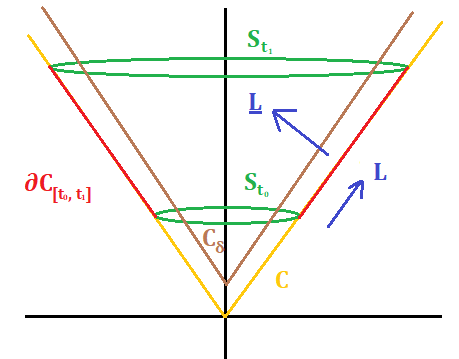
\includegraphics{graphics/cone}
			\caption{The geometry of the light cone. As a wise man once said, a picture is worth $\tfrac1\epsilon$-words for $\epsilon \ll 1$. }
		\end{center}	
	\end{figure}		

\subsubsection*{Subsets of $\R^d$ and $\R^{1 + d}$}
Define the restriction of the light cone to a time interval $I \subseteq [0, \infty)$ and a time slice $t \in [0, \infty)$ respectively by
	\begin{align*}
		C_I 
			&:= C \cap (I \times \R^d), \\
		S_{t}
			&:= C \cap (\{t\} \times \R^d).
	\end{align*}
The \emph{null boundary} $\partial C_I$ denotes the boundary of the time-slab $C_I$ modulo the top and bottom time-slices. Due to singularities on the null boundary, we will also consider the shifted light cone 
	\[ C^\delta := (\delta, 0) + C. \]
Accordingly, we have 
	\begin{align*}
		C^\delta_I
			&:= C_I \cap C^\delta, \\
		S^\delta_t
			&:= S_t \cap C^\delta.		
	\end{align*}	
We also define $B_r (x) \subseteq \R^d$ to be the ball of radius $r$ centered at $x$. 




\section{Outline of the proof}

Our overview of the argument follows the exposition of \cite{MR2528734}, which in turn outlines the stability result for $m \geq 4$ in \cite{gustafson2007schrodinger}; we will leave the modifications of the argument in \cite{GustafsonEtAl2010} to handle the $m = 3$ case to the details. For our notation, we will instead borrow from \cite[Geometric Wave Equations]{KochEtAl2014} and \cite{BejenaruTataru2014,bejenaru2024near}. 

We decompose the solution into a soliton profile and a dispersive error,
\begin{equation}\label{eq:decomp2}
	u(t, r) = \underbrace{Q_{\alpha(t), \lambda(t)}(r)}_{\text{modulated soliton}}  + \underbrace{\epsilon(t, r)}_{\text{dispersive error}} .
\end{equation}
To prove the main theorem, we want construct appropriate modulation parameters $(\alpha, \lambda)$ and correction term $\epsilon$ such that 
	\begin{enumerate}
		\item the error obeys global-in-time dispersive bounds, $\epsilon \in \mathsf S_{t, x}^1 ([0, \infty) \times \R^2)$, to obtain the dispersive decay, and \label{item:goal1}
		
		\item integrability bounds on the derivative of the modulation parameters, $(\dot {\alpha}, \dot{\lambda}) \in L^1_t ([0, \infty))$, to conclude convergence to a soliton. \label{item:goal2}
	\end{enumerate}
Here the $\mathsf S_{t, x}^1$-norm is taken to be a scale-invariant Strichartz-type norm at the level of the differentiated field $\partial u$. For our purposes, it will suffice to take the dispersive norm to consist of the endpoint norms, 
    \[
        ||\epsilon||_{\mathsf S_{t, x}^1} 
            := ||\epsilon||_{L^\infty_t \dot H^1_x} + || r^{-1}\epsilon ||_{L^2_t L^\infty_x}. 
    \]

\subsection{Generalised Hasimoto transformation}
	Generally, one would have to study the dynamics of the error coupled with the dynamics of the modulation parameters. However, the Schr\"odinger maps equation \eqref{schrodinger} admits \textit{self-dual} structure, which we first saw from the Bogomoln'yi identity \eqref{B}. Viewing the Schr\"odinger maps equation as the Hamiltonian flow of the Dirichlet energy, the Bogomoln'yi identity implies that the equation can be written as  
	\begin{equation}\label{eq:selfdual}
		\begin{split}
			\partial_t u 
				&= \bfJ \bfD_z \partial_{\overline z} u,
		\end{split}
	\end{equation}
    where 
    \begin{align*}
        \partial_{\overline z} u  
            &:= \partial_1 u - \bfJ \partial_2 u ,\\
        \bfD_z v 
            &:= \bfD_1 v + \bfJ \bfD_2 v. 
    \end{align*}
Then, applying the covariant Cauchy-Riemann operator to the self-dual formuation \eqref{selfdual}, we obtain the generalised Hasimoto-transformed Schr\"odinger maps equation, which is an elliptic-dispersive system,
    \begin{align}
        \bfD_t \epsilon'
            &= \bfJ \bfD_{\overline z} \bfD_z \epsilon' \label{eq:hasimoto2},\\
        \epsilon'
            &= \partial_{\overline z} u . \label{eq:hasimoto3}
    \end{align}
This is known as the \textit{generalised Hasimoto transformation}\footnote{The original Hasimoto transformation was derived in the context of fluids mechanics to transform the vortex filament equation into the one-dimensional cubic non-linear Schr\"odinger equation. The one-dimensional Schr\"odinger maps arises as the equation for the unit tangent field to the vortex filament. We point the interested reader to the classical book of Majda-Bertozzi \cite[Chapter 7.1]{MajdaBertozzi2002} for details. 
}, derived originally by Chang-Shatah-Uhlenbeck in \cite{ChangEtAl2000}. 
This formulation is convenient for two general reasons (see \cite[Chapter 6.2]{Tao2006} and \cite[Chapter 2.5]{KochEtAl2014} for more commentary on the \textit{frame method}) and one particular to the self-dual structure: 
    \begin{enumerate}
        \item the differentiated field takes values in a vector bundle $\epsilon' : I \times \R^2 \to u^* T \SS^2$ rather than a manifold like the original field $u: I \times \R^2 \to \SS^2$, so one can work in linear function spaces,
        
        \item we are free to choose an orthonormal frame for the bundle $u^* T\SS^2$ to concoct a favourable equation for $\epsilon'$ in coordinates, 
        
        \item in view of the harmonic maps equation \eqref{CR}, one can think of the map $u \mapsto \epsilon'$ as a non-linear projection which kills the harmonic maps component, leaving only the error, i.e. the differentiated field is at least linear in the error 
            \[
                \epsilon' = O(\epsilon) + O(\epsilon^2).
            \] 
        Thus we can view \eqref{hasimoto2} as a small $L^2_x$-data problem for a Schr\"odinger equation with cubic non-linear interactions. Using standard Strichartz estimates, it is well known that solutions to such equations admit global-in-time dispersive bounds $\epsilon' \in \mathsf S_{t, x}^0 ([0, \infty) \times \R^2)$. 
    \end{enumerate}
Our strategy then will be to prove dispersive estimates for the differentiated variable $\epsilon'$ using the non-linear Schr\"odinger equation \eqref{hasimoto2}. Using elliptic estimates for the inhomogeneous Cauchy-Riemann equation \eqref{hasimoto3}, we can pass these dispersive decay estimates onto the original error $\epsilon$. 
    \[
        ||\epsilon'||_{\mathsf S_{t, x}}
            := ||\epsilon'||_{L^\infty_t L^2_x} + || \epsilon'||_{L^2_t L^\infty_x}
    \]





\subsection{Orthogonality and modulation}

To identify the main enemy to proving decay estimates for the error, let us consider the linearisations of the Schr\"odinger maps equation \eqref{selfdual} and the Cauchy-Riemann equation \eqref{hasimoto3} about a fixed soliton profile $Q$. A solution to the linear flow is a field $u_{\mathrm{lin}} : I \times \R^2 \to Q^* T\SS^2$, which, upon choosing appropriate coordinates, e.g. Coulomb gauge $\{\vec v_Q, \vec w_Q \} \subseteq Q^* T\SS^2$, corresponds to a complex scalar field $\phi_{\mathrm{lin}} : I \times \R^2 \to \C$ satisfying 
    \begin{align}
        (i \partial_t - \mathsf{H}_Q) \phi_{\mathrm{lin}} \label{eq:linearised}
        &= N,\\
    \mathsf L_Q \phi_{\mathrm{lin}}
        &= F,\label{eq:linearisedCR}
    \end{align}
where $\mathsf H_Q$ is the \textit{linearised operator} and $\mathsf L_Q$ is the \textit{linearised Cauchy-Riemann operator}, given by 
\[
    \mathsf{H}_Q 
        := \mathsf{L}_Q^* \mathsf{L}_Q, 
        \qquad 
    \mathsf{L}_Q 
        := h_1 \partial_r {h_1}^{-1}.
\]
The factorisation of the linearised operator a l\'a the linearised Cauchy-Riemann operator can be read off from the self-dual structure of the equation. We see that the main enemy to decay of the error $\epsilon \approx \phi_{\mathrm{lin}}$, either via dispersive estimates from \eqref{linearised} or elliptic estimates from \eqref{linearisedCR}, would be the kernel of the linearised operators. From the perspective of the dispersive equation, the kernel elements lead to non-decaying, constant-in-time solutions, while from the perspective of the elliptic equation, the non-trivial kernel leads to non-uniqueness when attempting to invert the operator. 


\begin{figure}[h]\label{fig:orth}
    \begin{center}
        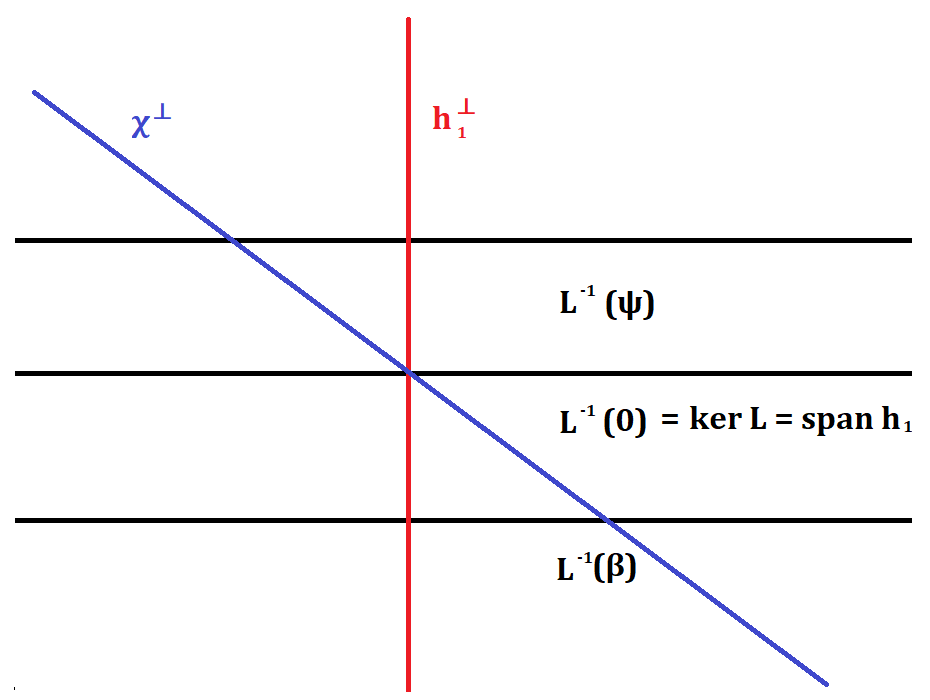
\includegraphics[scale = 0.4]{graphics/inverse}
        \caption{The level sets of the linear operator $\mathsf L_Q$ are affine subspaces of the domain which are parallel to the kernel 
            \[
            \mathsf L_Q^{-1} (\psi) = \phi + \ker \mathsf L_Q.
            \] 
        To identify a unique member $\phi$ in the level set, one must restrict the operator $\mathsf L_Q$ to a subspace which is transverse to the kernel. 
            }
    \end{center}    
\end{figure}

The kernel is given by 
\[
    \ker \mathsf{H}_Q = \ker \mathsf L_Q = \operatorname{span}_\C h_1.
\]
One can either read this off from the conjugation $\mathsf L_Q = h_1 \partial_r h_1^{-1}$ or invariance of the non-linear equations under scaling and rotation, which tells us that differentiating the modulated soliton $Q_{\alpha, \lambda}$ in these parameters generates elements of the kernel,
\begin{equation}\label{eq:generators}
    \begin{split}
    \frac{\partial Q_{\alpha, \lambda}}{\partial \alpha}\Big|_{(\alpha, \lambda) = (0, 1)}
        &= h_1 \vec v_Q,
        \\
    \frac{\partial Q_{\alpha, \lambda}}{\partial \lambda}\Big|_{(\alpha, \lambda) = (0, 1)} 
        &= h_1 
        \vec w_Q.
    \end{split}
\end{equation}

To kill these enemies, it will suffice to impose an orthogonality condition on the error, see Figure \ref{fig:orth}. 


Fix $\chi : (0, \infty ) \to (0, \infty)$ a radial, non-negative function which does not lie in the kernel, 
    \begin{equation}\label{eq:orthogonal1}
        \big\langle \epsilon, \chi^\lambda \big\rangle_{L^2_x} 
            = 0.
    \end{equation}
To enforce the orthogonality condition for all time, it suffices to solve the ODE furnished by differentiating the condition in time and imposing the condition holds initially at $t = 0$. This fixes the decomposition \eqref{decomp2}, as substituting it into the resulting ODE and using the equation \eqref{schrodinger} furnishes the \textit{modulation equation} for the parameters $(\alpha, \lambda)$. 

The linearised equations motivate two goals of the decomposition \eqref{decomp2},
\begin{enumerate}
    \item respects the linear flow \eqref{linearised},
    \item good elliptic estimates for the linearised Cauchy-Riemann operator \eqref{linearisedCR}. 
\end{enumerate}
Our first take would be to impose the condition that the error "$\epsilon \approx \phi$" is orthogonal to the kernel of the linearised operator $\mathsf H_Q$, 
\begin{equation}\label{eq:orthogonal}
    \phi_{\mathrm{lin}} \perp \ker \mathsf{H_Q} \qquad \text{"i.e."} \qquad \int_0^\infty \phi_{\mathrm{lin}} \, \overline{h_1} \, r dr 
        = 0. 
\end{equation}
This is a decomposition\footnote{Since the error is in the energy space, $\epsilon \in \dot H^1_m (\R^2)$, the orthogonality condition on the right is well-defined provided that $rh_1 \in L^2_r ([0, \infty))$ by Cauchy-Schwartz. The spatial asymptotics of the kernel elements are precisely $h_1 (r) = O(r^{-m})$, so one must restrict to the high equivariance case $m \geq 3$ to make sense of the orthogonality condition. } into invariant subspaces of the linearised flow, 
\[
    L^2_r ([0, \infty)) = \ker \mathsf H_Q \oplus (\ker \mathsf H_Q)^\perp.
\]
In view of the orthogonality of the error \eqref{orthogonal} to the generators of the kernel \eqref{generators}, the forcing terms in the modulation equations which are \textit{linear} in the error $\epsilon$ are killed, so
the derivatives of the parameters $(\dot{\alpha}, \dot{\lambda})$ only see \textit{quadratic} forcing terms and higher,
\begin{equation}\label{eq:quadratic}
    |\dot \alpha| + |\dot{\lambda}| 
        = O(|\epsilon|^2). 
\end{equation}
Thus, ignoring any technical problems with spatial asymptotics of $\epsilon$, an $L^2_t$-dispersive estimate for $\epsilon$ would imply an $L^1_t$-estimate for the parameters. This is favourable from the perspective of dispersive estimates, since our earlier discussion gives us access to $L^2_t L^\infty_x$-bounds on the differentiated error $\epsilon'$. At the level of the linearised Cauchy-Riemann operator, we would like to invert the operator and prove the fixed-time estimate 
    \[
        || r^{-1}\phi ||_{L^\infty_x} 
            \lesssim ||\mathsf L_Q \phi||_{L^\infty_x}.
    \]
By duality, one necessarily needs to place the function we are projecting away from in the dual space, i.e. we need $r \chi \in L^1_x (\R^2)$. In view of the asymptotics $h_1 = O(r^{-m})$, one necessarly needs $m \geq 4$. To reach $m = 3$, we need to replace our orthogonality condition with a generic test function $\chi \in C^\infty_c (0, \infty)$; this price one pays is that the linearised flow \eqref{linearised} no longer preserves the decomposition, so $(\dot{\alpha}, \dot{\lambda})$ are forced by linear terms in $\epsilon$ in the modulation equations,
    \[
        |\dot{\alpha}| + |\dot{\lambda}| 
            = O(\epsilon) + O(\epsilon^2). 
    \]
To handle the linear terms, we make a \textit{normal form transformation}.






\section{Elliptic estimates}



To pass the dispersive bounds on the differentiated field $\epsilon'$ back onto the error $\epsilon$, we need to prove appropriate non-linear elliptic estimates for non-linear Cauchy-Riemann operator relating the two fields via \eqref{hasimoto3}, i.e. we study the equation 
    \begin{equation}\label{eq:CR3}
        \epsilon' 
            =\partial_{\overline z} u ,
    \end{equation}
where the Cauchy-Riemann operator acts on $m$-equivariant fields by 
    \[
        \partial_{\overline z} u 
            := \partial_r u - \frac{m}{r} u \times Ru.
    \]
Recall the linearised operator takes the form   
    \[
        \mathsf L_u \phi 
            :=  u_1 \partial_r {u_1}^{-1}.
    \]

\subsection{Linearised equation}

To identify the main terms, we linearise the equation by decomposing the error into a component perpindicular to the soliton profile (i.e. in the tangent space $T_Q \SS^2$) and a component parallel to the soliton profile, 
\begin{equation}\label{eq:perpparallel}
    \begin{split}
        u(t, r) 
            &=  \underbrace{Q(r)}_{\text{soliton profile}} + \underbrace{\epsilon(t, r)}_{\text{perturbation}} \\
            &= \underbrace{Q(r)}_{\text{soliton profile}} + \underbrace{u_{\mathrm{lin}} (t, r)}_{\text{perpindicular perturbation}} + \underbrace{\gamma(t, r) Q(r)}_{\text{parallel perturbation}}
    \end{split}
\end{equation}
For the more visually-inclined reader, see Figure \ref{fig:decomp} below, 

\begin{figure}[h]
\begin{center}
    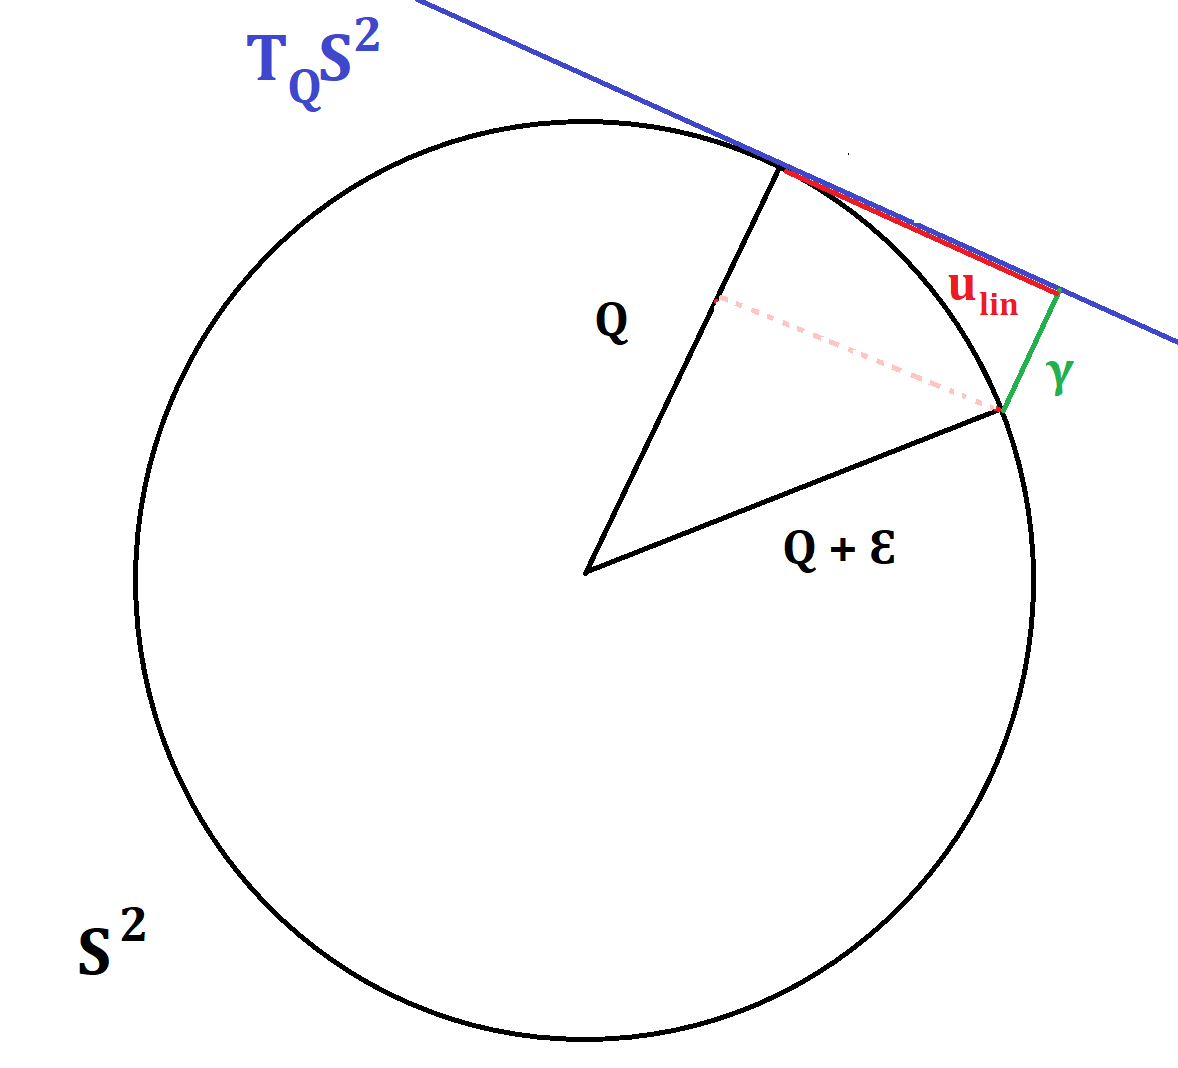
\includegraphics[scale = 0.3]{graphics/coulombQ}
    \caption{Decomposition of the error 
        \[\epsilon = u_{\mathrm{lin}} + \gamma Q,\] 
    into a component parallel to the soliton $\gamma Q \in \operatorname{span} Q$ and a component in the tangent space $u_{\mathrm{lin}} \in T_Q \SS^2$. For small error, the main term is the latter. }\label{fig:decomp}
\end{center}
\end{figure}

For small perturbation $|\epsilon| \ll 1$, the main term in the decomposition \eqref{perpparallel} is the perpindicular component $\epsilon \approx u_{\mathrm{lin}}$ in view of the constraint $|u| \equiv |Q| \equiv 1$; indeed one can compute that the parallel part is of quadratic order in $\epsilon$, 
\begin{align*}
    \gamma 
        &= \sqrt{1 - |u_{\mathrm{lin}}|^2} - 1 = O(|u_{\mathrm{lin}}|^2).
\end{align*}
Analogous to the study of the dispersive equation \eqref{hasimoto2}, we would like to fix a coordinate system which reveals the elliptic structure of the equations \eqref{hasimoto3} and furthermore is well-adapted to the decomposition \eqref{perpparallel}. In this case, we choose the Coulomb frame $\{\vec v_Q, \vec w_Q \} \subseteq Q^* T\SS^2$ adapted to the soliton profile $Q$, which takes the explicit form 
\begin{equation}\label{eq:coulombQframe}
        \vec v_Q (r) 
            = \begin{pmatrix} h_3 (r) \\ 0 \\ - h_1 (r) \end{pmatrix},
        \qquad
        \vec w_Q (r) 
            = \begin{pmatrix} 0 \\ 1 \\ 0 \end{pmatrix}. 
\end{equation}
In these coordinates, the fields $u_{\mathrm{lin}} : I \times \R^2 \to Q^* T\SS^2$ and differentiated field $\epsilon' : I \times \R^2 \to u^* T\SS^2$ correspond respectively to the complex scalar fields $\phi : I \times \R^2 \to \C$ and $\widetilde{\psi} : I \times \R^2 \to \C$, defined by 
    \begin{align*}
        \phi
            &:= \big\langle  u_{\mathrm{lin}}, \vec v_Q \big\rangle + i \big\langle u_{\mathrm{lin}}, \vec w_Q \big\rangle,\\
        \widetilde{\psi} 
            &:= \big\langle  \epsilon' , \vec v_Q \big\rangle + i \big\langle \epsilon', \vec w_Q \big\rangle.
    \end{align*}
Using the decomposition \eqref{perpparallel}, we can write the  inhomogeneous Cauchy-Riemann equation \eqref{CR3} in the Coulomb frame as 
\begin{equation}\label{eq:CRcoulomb}
    \underbrace{\mathsf L_Q \phi}_{\text{linearised operator}} 
        = \underbrace{\widetilde{\psi}}_{\text{dispersive bound}} - \underbrace{\frac{m}{r} \epsilon_3 \phi + \frac{m}{r} h_1 \gamma}_{\text{perturbative non-linearity}}. 
\end{equation}    
Thus, we see that, at least on the linear level, passing bounds on the differentiated field $\widetilde{\psi}$ to the main error $\phi$ amounts to inverting the linearised operator $\mathsf L_Q$. 

\subsection{Elliptic estimates}

The right-inverse is given by 
    \[
        \mathsf R_\chi g (r) 
            := 2\pi h_1 (r) \int_0^\infty \left( \int_{r'}^r h_1(r'') g(r'') dr'' \right) \overline{\chi (r')} h_1 (r') \, r' dr'.  
    \]

\begin{lemma}[Linear elliptic estimate]\label{lem:linearelliptic}
    For each $\lambda > 0$ and radial function $\chi : (0, \infty) \to (0, \infty)$, there exists a linear operator $\mathsf R_{\lambda, \chi}$ which serves as a right-inverse for $\mathsf L^\lambda$ and also a left-inverse for $\mathsf L_{\lambda}$ modulo the kernel, 
        \begin{align}
            \mathsf L^\lambda \mathsf R^\lambda_{\chi} g 
                &= g, \\
            \mathsf R^\lambda_{\chi} \mathsf L^\lambda g
                &= g - h_1 (r/\lambda) \int_0^\infty g (r')\overline{\tfrac{1}{\lambda^2} \chi \big( \tfrac{r}{\lambda}\big)} r' dr'.
        \end{align}
Furthermore, for $1 \leq p \leq \infty$ and $|\theta| < m$, if $\chi \in r^{-1} (\ell^{p'} L^1)_x (0, \infty)$, then the right-inverse satisfies the bound
        \begin{equation}
            || r^{-\theta} \mathsf R^\lambda_{\chi} g ||_{(\ell^p L^\infty)_x} 
                \lesssim || r^\theta \chi||_{ (\ell^{p'}L^1)_x} || r^{-\theta - 1}g||_{ (\ell^p L^1)_x}
        \end{equation}
\end{lemma}

\begin{proof}
    Note that 
        \[
            g(r) 
                \mapsto g\big(\tfrac{r}\lambda\big), \qquad
            \chi(r) 
                \mapsto \tfrac{1}{\lambda^2} \chi \big( \tfrac{r}{\lambda}\big)
        \]
    are adjoint operators, so it suffices to prove the result for $\lambda = 1$. For the details, we refer the reader to \cite[Section 10.1]{GustafsonEtAl2010}. 
\end{proof}

\begin{proposition}[Non-linear elliptic estimates]
    For $m \geq 2$, consider the inhomogeneous non-linear Cauchy-Riemann equation \eqref{CRcoulomb}. If the error satisfies the orthogonality condition 
        \begin{equation}\label{eq:ellipticorthogonal}
            \int_0^\infty \phi (r) \overline{\widetilde{h_1}(r/\lambda)} \, r dr 
                = 0,
        \end{equation}
    where $\widetilde{h_1} \in C^\infty_c (0, \infty)$ is a smooth compactly-supported radial function satisfying $\langle h_1, \widetilde{h_1} \rangle_{L^2_r} = 1$, then 
        \begin{enumerate}
            \item $L^2_x$-type bound 
                \begin{equation}
                    ||\phi||_{\dot H^1_m}    
                        \lesssim || \psi ||_{L^2_r} + ||\phi||_{L^\infty_r} ||\phi||_{\dot H^1_m}, \label{eq:ellipticenergy}
                \end{equation}

            \item $L^\infty_x$-type bound
                \begin{equation}
                    ||r^{-1} \phi ||_{(\ell^p L^\infty)_r} 
                        \lesssim ||\psi ||_{L^\infty_r} + ||\phi||_{L^\infty_r} ||\phi||_{(\ell^p L^\infty)_r}.\label{eq:ellipticuniform}
                \end{equation}
        \end{enumerate}
 \end{proposition}

\begin{proof}
    By the orthogonality condition \eqref{ellipticorthogonal}, we have 
        \[
            \phi 
                = \mathsf R_{\lambda, \widetilde{h_1}} \mathsf L^\lambda \phi. 
        \]
    The equation \eqref{CRcoulomb} schematically takes the form 
        \[
            \mathsf L_Q \phi  
                = \widetilde{\psi} + O(|\phi|^2).
        \]
    Using the estimates from Lemma \ref{lem:linearelliptic} and the triangle inequality, placing one factor of $\phi$ in the non-linearity in $L^\infty_r$-norm and the other in either $\dot H^1_m$-norm or $(\ell^p L^\infty)_r$-norm, furnishes the $L^2_x$-bound and $L^\infty_x$-bound respectively. 
\end{proof}


\begin{proposition}[Hardy-Sobolev inequality]
    Let $m \geq 1$ and suppose $\phi \in \dot H^1_m (0, \infty)$ is $m$-equivariant, then 
        \begin{equation}
            ||\phi||_{L^\infty_r}
                \lesssim ||\phi||_{\dot H^1_m}\label{eq:elliptichardy}.
        \end{equation}
\end{proposition}

\begin{proof}
    Fundamental theorem of calculus and Cauchy-Schwartz. 
\end{proof}

\section{Dispersive estimates}

To prove dispersive bounds for the differentiated field $\epsilon'$, we fix a gauge to write \eqref{hasimoto2} as a cubic non-linear Schr\"odinger equation with potential. Using standard arguments, one can prove Strichartz estimates for the linearised equation, and, in view of the small data assumption, the non-linearity is perturbative. Again, the equation we consider is 
    \begin{equation}\label{eq:hasimotodisp}
        \bfD_t \epsilon' 
            = \bfD_z \bfD_{\overline z} \epsilon'. 
    \end{equation}

\subsection{Linearised equation}

To reveal the Schr\"odinger structure of the equation, we work in coordinates, fixing an $m$-equivariant frame $\{\vec v, \vec w\} \subseteq u^* T\SS^2$. Using this frame, we can identify the differentiated field $\epsilon' : I \times \R^2 \to u^* T\SS^2$ with the complex scalar field $\psi: I \times \R^2 \to \C$ via 
    \begin{align*}
        \psi 
            &:= \big\langle \epsilon', \vec v \big\rangle + i \big\langle \epsilon', \vec w \rangle.
    \end{align*}
The connection coefficients are given by
    \begin{align*}
        A_t 
            &= \big\langle \partial_t \vec v, \vec w \big\rangle, \\
        A_r 
            &= \big\langle \partial_r \vec v, \vec w \big\rangle, \\
        A_r 
            &= \big\langle \partial_\theta \vec v, \vec w \big\rangle.
    \end{align*}



\begin{proposition}[Hasimoto transform in Coulomb gauge]
    Let $u : I \times \R^2 \to \SS^2$ be a solution to Schr\"odinger maps \eqref{schrodinger}, and denote $\{\vec v, \vec w\} \subseteq u^* T\SS^2$ the frame satisfying the Coulomb gauge condition 
        \begin{equation}
            \begin{split}
                \partial_1 A_1 + \partial_2 A_ 2 
                    &= 0.
            \end{split}
        \end{equation}
    Then the connection coefficients are given by  
        \begin{align}
            A_r [u] 
                &= 0,\\
            A_\theta [u]
                &= m u_3,\\
            A_t [u]
                &=A_t [u] 
                = \left( \frac12|\epsilon'|^2 + \frac{m}{r} \epsilon_3'\right) + \int_r^\infty 2 \left( \frac12|\epsilon'|^2 + \frac{m}{r'} \epsilon_3' \right) \frac{dr'}{r'}.
        \end{align}
\end{proposition}

\begin{proof}
\leavevmode
    \begin{enumerate}
        \item In polar coordinates, the Coulomb gauge condition reads 
            \[
                \partial_r A_r + \frac{1}{r^2} \partial_\theta A_\theta = 0. 
            \]
        Since the connection coefficients are radial and satisfy appropriate boundary conditions at infinity, we immediately conclude $A_r = 0$. 

        \item Since $\vec v$ and $\vec w$ are equivariant and $\{u, \vec v, \vec w\} \subseteq \R^3$ are orthonormal vectors, 
            \begin{align*}
                A_\theta    
                    &= \partial_\theta \vec v \cdot \vec w \\\
                    &= (m\vec k \times \vec v) \cdot \vec w \\
                    &= m \vec k \cdot (\vec v \times \vec w) = m\vec k \cdot \vec u = m u_3. 
            \end{align*}
        \item Exercise. 
    \end{enumerate}
\end{proof}

The equation takes the form  
\begin{equation}
    (\partial_t + i A_t[u]) \psi 
        = -i \mathsf L_u \mathsf L^*_u \psi. 
\end{equation}
Expanding, and regarding the modulation as slow and thus the differences in some terms in the potential as perturbative, we can write 
\begin{equation}\label{eq:hasimotoS}
    \begin{split}
        (i \partial_t - \widetilde{\mathsf H}_Q) \psi 
            &= \cN_1 + \cN_2 + \cN_3,
    \end{split}
    \end{equation}
where the main linear part is given by 
\begin{align*}
    \widetilde{\mathsf H}_Q 
        &:= - \Delta + \widetilde{V}_Q,\\
    \widetilde{V}_Q (r)
        &:= \frac{2m(1 - h_3(r))}{r^2} = \frac{4m}{r^2 (r^2 + 1)}
\end{align*}
and the pertubrative part is given by 
\begin{align*}
        \cN_1 
            &:=  i A_t[u] \psi,\\
        \cN_2
            &:= - 2i m \frac{h_3 - h_3^\lambda }{r^2} \psi \\
        \cN_3 
            &:= - 2i m \frac{\epsilon_3}{r^2} \psi - i m \frac{\epsilon_3'}{r}\psi.
    \end{align*}
We can estimate the perturbative terms in the dual Strichartz space 
    \begin{align}
        ||\cN_1||_{L^2_t (\ell^2 L^1)_x}
            &\lesssim  ||\psi||_{L^2_t (\ell^2 L^\infty)_x}^2,\\
        ||\cN_2||_{L^2_t (\ell^2 L^1)_x}
            &\lesssim \left|\left|h_3 \big(\tfrac{\lambda(t)}{\lambda(0)}\big)\right|\right|_{L^\infty_t}  ||\psi||_{L^2_t (\ell^2 L^\infty)_x}\\
            ||\cN_3||_{L^2_t (\ell^2 L^1)_x}
            &\lesssim ||\psi||_{L^2_t (\ell^2 L^\infty)_x}^2.
    \end{align}
In the case of the linear term $\cN_2$ we assume $\lambda$ is slowly varying to regard this term as perturbative; this is the main goal of the modulation theory. 

\subsection{Strichartz estimates}

We want to prove a Strichartz estimate for a Schr\"odinger equation with potential. More generally, one can regard this is a variable-coefficient Schr\"odinger equation. Let us begin with some generalities; consider a self-adjoint Schr\"odinger operator $\mathsf H$, and its corresponding linear flow 
    \begin{equation}\label{eq:generic}
        \begin{split}
            (i \partial_t - \mathsf H) \psi 
                &= f,\\
            \psi_{|t = 0}
                &= \psi_0.  
        \end{split}
    \end{equation}
We say that $\mathsf H$ satisfies the \textit{(double) endpoint Strichartz estimate} if 
    \begin{equation}\label{eq:strichartz}\tag{S}
        ||\psi||_{L^2_t (\ell^2 L^\infty)_x}    
            \lesssim ||\psi_0||_{L^2_r} + ||f||_{L^2_t (\ell^2 L^1)_x}.
    \end{equation}
In view of the bounds on the non-linearity in the dual space and assuming the scaling parameter is slowly moving $|\log(\lambda/\lambda_0)|\ll 1$, the right-hand side can be regarded as perturbative and we conclude the dispersive estimate 
    \begin{equation}\label{eq:dispersive}
        ||\psi||_{L^\infty_t L^2_x \cap {L^2_t (L^\infty_2)_x}} 
            \ll 1. 
    \end{equation}

The standard proof of the Strichartz estimate for the Laplacian $\mathsf H = -\Delta$ relies on the explicit kernel for the linear propagator $e^{it \Delta}$ and the method of stationary phase. This method is unfortunately not very robust, as classical Fourier analysis is ill-suited for variable-coefficient operators. Instead, we will rely on a weaker form of dispersion as a stepping stone for proving \eqref{strichartz}; we say $\mathsf H$ satisfies \textit{integrated local energy decay} (also known as the \textit{local smoothing estimate}) if 
    \begin{equation}\label{eq:ILED}\tag{ILED}
        ||r^{-1} \psi||_{L^2_{t, x}}
            \lesssim ||\psi_0||_{L^2_x} + ||r f||_{L^2_{t, x}}.
    \end{equation}
The heuristic is as follows; given a wave packet $\psi$ localised to frequency $|\xi| \approx N$, the packet travels under a homogeneous Schr\"odinger-type flow with group velocity $|v| \approx N$. Thus for a compact region $K \subseteq \R^2$ of radius $R$, the bulk of the mass only remains in the region for time scale $T \approx R/N$, so integrating-in-time the mass in the fixed region gives
    \[
        \int_\R \int_K |\psi|^2 \, dx dt 
            \lesssim \frac{R}{N} \int_{\R^2} |\psi|^2 \, dx. 
    \]
This represents a \textit{gain} of $\tfrac12$-derivatives on the left-hand side after localising-in-space and averaging-in-time. The proof is more robust, using little more than integration-by-parts (in the form of the \textit{positive commutator method}). Furthermore, in the time-independent case $\mathsf H(t) \equiv \mathsf H$, the problem can be further reduced to studying the spectral properties of the operator. 

Our strategy can then be summarised as follows:
    \[
       \text{\eqref{strichartz} for $\Delta$} +\text{\eqref{ILED} for $\mathsf H_Q$} \implies \text{\eqref{strichartz} for $\mathsf H_Q$}
    \]


\begin{lemma}[Endpoint Strichartz for $m$-equivariant Laplacian]
    The endpoint Strichartz estimate \eqref{strichartz} holds for $\mathsf H = - \Delta$ upon restricting to the class of $m$-equivariant functions for $m \geq 1$. 
\end{lemma}

\begin{proof}
    C.f. \cite[Theorem 10.1]{GustafsonEtAl2010}.
\end{proof}

\begin{remark}
    In the case of radial functions $m = 0$, the homogeneous Strichartz estimate holds for the Laplacian, however, the inhomogeneous estimate fails, c.f. the classical paper of Tao \cite{tao2000spherically}. 
\end{remark}

\begin{lemma}[ILED implies Strichartz]
    Let $\mathsf H_0$ be a self-adjoint operator for which the endpoint Strichartz estimate \eqref{strichartz} holds, and consider the Schr\"odinger operator with potential $\mathsf H := \mathsf H_0 + V$. If $V(x)$ is a real-valued potential satisfying the growth condition 
        \begin{equation}\label{eq:growth}
            \sup_{x \in \R^2} |x|^2 |V(x)|
                < \infty, 
        \end{equation}
    and integrated local energy decay \eqref{ILED} holds for $\mathsf H$, then the endpoint Strichartz estimate \eqref{strichartz} also holds for $\mathsf H$. 
\end{lemma}

\begin{proof}
    We can rewrite the equation for the operator with potential as 
        \begin{align*}
            (i \partial_t - \mathsf H_0)\psi
                &= f + V \psi,\\
            \psi_{|t = 0}
                &= \psi_0. 
        \end{align*} 
    Applying Strichartz for $\mathsf H_0$, the growth condition \eqref{growth}, and integrated local energy decay \eqref{ILED}, and the embedding 
        \begin{align*}
            ||\psi||_{L^2_t (\ell^2 L^\infty)_x}
                &\lesssim ||\psi_0||_{L^2_x} + ||f||_{L^2_t (\ell^2 L^1)_x} + ||V\psi||_{L^2_t (\ell^2 L^1)_x}\\
                &\lesssim ||\psi_0||_{L^2_x}  + ||f||_{L^2_t (\ell^2 L^1)_x} + \big|\big| r^2 V\big|\big|_{L^\infty_x} \big|\big| r^{-1}\psi\big|\big|_{L^2_{t, x}}\\
                &\lesssim  ||\psi_0||_{L^2_x}  + \big|\big| r f\big|\big|_{L^2_{t, x}} .
        \end{align*}
    By duality, 
        \[
            || r^{-1}\psi||_{L^2_{t, x}} 
                \lesssim ||\psi_0||_{L^2_x} +  ||f||_{L^2_t (\ell^2 L^1)_x.}.
        \]
    Feeding this into the second line of the previous inequality finishes the proof. 
\end{proof}

\begin{proposition}
    Let $V \in C^1_r (0, \infty)$ be a radial real-valued potential satisfying the growth condition \eqref{growth} along with the conditions
        \begin{align}
            \inf_{r > 0} r^2 V(r) 
                &> 0,\\
            \inf_{r > 0} - r^2 \partial_r (r V(r)) 
                &> 0.
        \end{align}
    Then the Laplacian with potential $\mathsf H := - \Delta + V$ satisfies both integrated local energy decay \eqref{ILED} and the endpoint Strichartz estimate \eqref{strichartz} in the class of $m$-equivariant functions. 
\end{proposition}

\begin{proof}
    See Burq-Planchon-Stalker-Tahvildar-Zadeh \cite{BurqEtAl2004}. The proof boils down to proving the resolvent satisfies the uniform bounds
        \begin{equation}
            \sup_{\lambda \neq 0}  
                ||(\mathsf H - \lambda)^{-1} f||_{\mathsf{LE}_{x}} 
                    \lesssim ||f||_{\mathsf{LE}^*_x}.
        \end{equation}
    To see how this is sufficient, we point the interested reader to \href{https://github.com/zhao-j4/notes/blob/main/seminar%20notes/local%20energy%20decay/main.pdf}{our notes on the wave case}. 
\end{proof}

\subsection{Dispersive decay}

Use the Fraunhofer formula, dispersive bounds \eqref{dispersive} and the elliptic bounds \eqref{ellipticenergy}-\eqref{ellipticuniform}, we can prove 
    \begin{equation}
        ||\phi||_{L^\infty_x} \overset{t \to \infty}{\longrightarrow} 0 . 
    \end{equation}


\section{Modulation theory}

It remains to show that the modulation parameters converge $(\lambda(t), \alpha(t)) \to (\lambda_\infty, \alpha_\infty)$. Our strategy will be to show suitable $L^1_t$-bounds for the perturbative part of the equation for the derivatives $(\dot{\lambda}, \dot{\alpha})$, and rewrite the non-perturbative part as a total derivative. To derive the modulation equations, recall that the Schrodinger maps equation can be written using the decomposition as 
    \begin{equation}\label{eq:schromod}
        \partial_t \epsilon 
            = \partial_t u - \partial_t Q_{\alpha(t), \lambda(t)} = -\bfD_z \epsilon' - h_1^\lambda (\vec v_Q + \vec w_Q) \dot{\mu}. 
    \end{equation}
Then, writing in coordinates, and then integrating against $\widetilde{h_1}$, using the orthogonality condition \eqref{orthogonal1} to kill the left-hand side, we obtain the modulation equation 
    \begin{equation}\label{eq:modulate1}
        \dot{\mu} 
            = - i \big\langle \mathsf L_u^* \psi, \tfrac{1}{\lambda^2} \widetilde{h_1}^\lambda \big\rangle_{L^2_x} + \text{higher order terms}.
    \end{equation}
If we had $h_1$ instead of $\widetilde{h_1}$, then the linear term would vanish up to terms which are higher order. Unfortunately, we must contend with this term if we want to pass good $L^\infty_x$ estimates from $\epsilon'$ onto $\epsilon$. Let us disregard the higher order terms, one has 
    \[
        ||\text{higher order} ||_{L^1_t} \lesssim ||\psi||_{L^2_t L^\infty_x}^2.
    \]
Since $h_1$ is in the kernel of $\mathsf L_Q$, we can test the equation \eqref{schromod} against $h_1$, and compare against what we obtained for the modulation equation \eqref{modulate1}. 
    \[
        \dot{\mu} 
            =- i \big\langle \mathsf L_u^* \psi, \tfrac{1}{\lambda^2} (\widetilde{h_1}^\lambda - c h_1^\lambda) \big\rangle_{L^2_x} + \text{higher order terms}
    \]
The difference between testing against $\widetilde{h_1}$ and $h_1$ is as follows; let $c = ||h_1||_{L^2}^{-2}$, then 
    \[
        \langle \widetilde{h_1} - c h_1, h_1 \rangle = 1 - c ||h_1||_{L^2}^2 = 0. 
    \]
This tells us that $\widetilde{h_1} - c h_1 \perp \ker \mathsf L_Q$, so it follows that one can write 
    \[
        \widetilde{h_1} - c h_1 = L^*_Q R^*_{\widetilde{h_1}} (\widetilde{h_1} - c h_1) =: L_Q^* g . 
    \]
Thus we can rewrite the linear term, using the equation \eqref{hasimotodisp},
    \[
        \big\langle \mathsf L_u^* \psi, \tfrac{1}{\lambda^2} (\widetilde{h_1}^\lambda - c h_1^\lambda) \big\rangle_{L^2_x} = \big\langle \mathsf L_u^* \psi, \tfrac{1}{\lambda} L_Q^* g \big\rangle_{L^2_x} = \big\langle \partial_t \psi, \tfrac{1}{\lambda} g \big\rangle_{L^2_x} + \text{higher order}. 
    \]
Now we can differentiate by parts in time to recover a full derivative, plus some terms which are higher-order. For the remainder of the proof, see \cite[Section 7, 8]{GustafsonEtAl2010}.

\appendix

\section{}
\subsection{Generalised Hasimoto transform}\label{appendix:hasimoto}

It is convenient to write the Schr\"odinger maps equation \eqref{schrodinger} in geometric formulation, 
    \[
        \partial_t u 
            = \bfJ (\bfD_1 \partial_1 u + \bfD_2 \partial_2 u). 
    \]  
Then 
    \begin{align*}
        \bfJ \bfD_z \partial_{\overline z} u 
            &= \bfJ (\bfD_1 + \bfJ \bfD_2) (\partial_1 u - \bfJ \partial_2 u) \\
            &= \bfJ (\bfD_1 \partial_1 u - \bfJ \bfJ \bfD_2 \partial_2 u) + \bfJ\bfJ (\bfD_1 \partial_2 u - \bfD_2 \partial_1u)\\
            &= \bfJ (\bfD_1 \partial_1 u + \bfD_2 \partial_2 u).
    \end{align*}


\subsection{Bogomoln'yi identity}\label{appendix:bogo}

We compute
    \begin{align*}
        |\partial_1 u - u \times \partial_2 u |^2 
            &= (\partial_1 u - u \times \partial_2 u) \cdot (\partial_1 u - u \times \partial_2 u)\\
            &= |\partial_1 u|^2 + |u \times \partial_2 u|^2 - 2 (\partial_1 u) \cdot (u \times \partial_2 u) .
    \end{align*}
In the last line, the first two terms are exactly the Dirichlet energy density, while the last term is the pull-back of the volume form on $\SS^2$ to $\R^2$ under $u$. Indeed, since the almost complex structure acts isometrically on the tangent space,    
    \[
        |\partial_1 u|^2 + |u \times \partial_2 u|^2 = |\partial_1 u|^2 + |\partial_2 u|^2. 
    \]
To see the pull-back of the volume form, recall that 
    \[
        d\operatorname{Vol}_{\SS^2}
            := u^1 du^2 \wedge du^3 - u^2 du^1 \wedge du^3 + u^3 du^1 \wedge du^2.
    \]
Then, pulling back by $u : \R^2 \to \SS^2$, we obtain 
    \begin{align*}
        u^* d \operatorname{Vol}_{\SS^2}
            &= u^1 (\partial_1 u^2 dx^1 + \partial_2 u^2 dx^2) \wedge  (\partial_1 u^3 dx^1 + \partial_2 u^3 dx^2) \\
            &\qquad - u^2 (\partial_1 u^1 dx^1 + \partial_2 u^1 dx^2)  \wedge (\partial_1 u^3 dx^1 + \partial_2 u^3 dx^2)  \\
            &\qquad + u^3 (\partial_1 u^1 dx^1 + \partial_2 u^1 dx^2)  \wedge  (\partial_1 u^2 dx^1 + \partial_2 u^2 dx^2) \\
            &= u \cdot (\partial_1 u \times \partial_2 u) \, dx^1 \wedge dx^2\\
            &=  (\partial_1 u) \cdot (u \times \partial_2 u) \, dx^1 \wedge dx^2, 
    \end{align*}
where the last line we have used the scalar triple product identity. By the degree theorem, 
    \begin{align*}
        \int_{\R^2} (\partial_1 u) \cdot (u \times \partial_2 u) \, dx
            &= \int_{\R^2} u^* d\operatorname{Vol} = \deg(u) \int_{\SS^2} d\operatorname{Vol} = 4\pi  \deg(u)
    \end{align*}
This completes the proof of the Bogomoln'yi identity \eqref{B}. 


\subsection{Harmonic maps from \eqref{LL}}

Here we show that 
    \[
        \partial_t u 
            = \alpha( \Delta u + |\nabla u|^2 u) + \beta (u \times \Delta u)
    \]
is equivalent to 
    \[
        \partial_t u 
            = -\alpha (u \times (u \times \Delta u)) + \beta (u \times \Delta u ).
    \]
Consider the vector cross product formula 
    \[
        a \times (b \times c) = (a \cdot c) b - (a \cdot b) c. 
    \]
Then 
    \[
        u \times (u \times \Delta u) = (u \cdot \Delta u) u - |u|^2 \Delta u. 
    \]
Observe that 
    \[
        u \cdot \nabla u = 0. 
    \]
Thus 
    \[
        u \cdot \Delta u = - |\nabla u|^2. 
    \]

\bibliographystyle{alpha}
\bibliography{external/biblio}

\end{document}
